\documentclass[a4paper,12pt]{scrreprt}

\usepackage[italian]{babel}

\usepackage[utf8]{inputenc}

\usepackage{mathtools}
\DeclarePairedDelimiter{\ceil}{\lceil}{\rceil}

\usepackage{graphicx}
\graphicspath{{images/}}

\usepackage{tcolorbox}
\tcbuselibrary{theorems,minted,breakable}
\newtcbtheorem[number within=chapter]{mynote}{Nota}{%
  colback=blue!5,
  colframe=blue!35!black,
  breakable,
  fonttitle=\bfseries,
  before={\vspace{0.5cm}},
  after={\vspace{0.5cm}}}{note}
\newtcblisting{myvhdl}[1]{%
  listing only,
  minted language=vhdl,
  minted options=breaklines,
  fonttitle=\bfseries,
  before={\vspace{0.5cm}},
  after={\vspace{0.5cm}},
  breakable,
  title=#1
}
\newcommand{\BashFancyFormatLine}{%
  \def\FancyVerbFormatLine##1{\$\,##1}%
}
\newtcblisting{commandshell}{%
  colback=black,
  colupper=white,
  breakable,
  colframe=yellow!75!black,
  listing only,
  before={\vspace{0.5cm}},
  after={\vspace{0.5cm}},
  minted options={formatcom=\BashFancyFormatLine}}

\usepackage{hyperref}

\usepackage{courier}
\usepackage{listings}
\lstset{
  basicstyle=\ttfamily,
  breaklines=true
}

\title{Il Processore Mic-1 \\
  \ \\
  \large Dispensa didattica del corso di\\
  Architettura dei Sistemi di Elaborazione}
\author{Prof.\ Nicola Mazzocca \\
  Ing.\ Alberto Moriconi}
\date{}

\begin{document}
\maketitle

\chapter{Il Livello Microarchitetturale}

Il processore Mic-1 è un utile esempio didattico, presentato in~\cite{tanenbaum}
per due scopi principali:
\begin{enumerate}
  \item mostrare come, usando elementi logici di base come quelli già studiati
  nel corso, sia possibile realizzare una microarchitettura che implementi un
  semplice set di istruzioni;
  \item mostrare come anche la realizzazione di un sistema apparentemente
  complesso, come un processore, si riduca in realtà alla progettazione di
  un'unità operativa e di un'unità di controllo, e del modo in cui devono
  comunicare.
\end{enumerate}

Il set di istruzioni implementato dal Mic-1 è un sottoinsieme di quello della
Java Virtual Machine, denominato \textit{IJVM} in quanto opera unicamente sugli
interi.

Una particolarità di questo processore è quella di non disporre di registri
generali; la sua architettura è infatti di tipo \textit{a stack}: le sue
istruzioni aritmetiche e logiche non hanno operandi espliciti, ma li prelevano
da una struttura \textit{last-in-first-out} allocata nella memoria principale,
in cui devono essere posti in precedenza.

\medskip

Per iniziare a comprendere come opera un processore di questo tipo, consideriamo
ad esempio l'esecuzione dell'operazione di somma e assegnazione

\begin{tcblisting}{listing only}
  a1 = a2 + a3
\end{tcblisting}

che è tradotta in linguaggio assembly IJVM come

\begin{tcblisting}{listing only}
  ILOAD a2
  ILOAD a3
  IADD
  ISTORE a1
\end{tcblisting}

Lo stato dello stack durante l'esecuzione evolve come in
fig.~\ref{fig:stack_add}; inizialmente, le locazioni di memoria \lstinline{a2} e
\lstinline{a3} contengono gli operandi, mentre la locazione \lstinline{a1} è non
inizializzata; dunque:
\renewcommand{\labelenumi}{(\alph{enumi})}
\begin{enumerate}
  \item la prima istruzione \lstinline{ILOAD} legge il contenuto della locazione
  di memoria \lstinline{a2} e ne esegue il push su stack;
  \item la seconda istruzione \lstinline{ILOAD} legge il contenuto della
  locazione di memoria \lstinline{a3} e ne esegue il push su stack;
  \item l'istruzione \lstinline{IADD} esegue il pop dei due elementi in cima
  allo stack e il push della loro somma;
  \item l'istruzione \lstinline{ISTORE} esegue il pop della somma e la scrive in
  memoria alla locazione \lstinline{a1}.
\end{enumerate}
\renewcommand{\labelenumi}{\arabic{enumi}.}

\begin{figure}
  \centering
  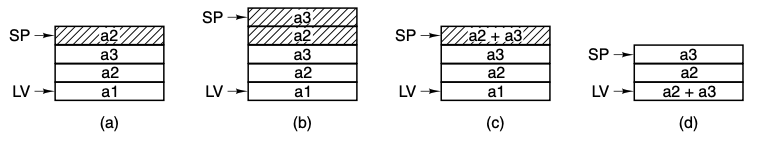
\includegraphics[width=\textwidth]{stack_add.png}
  \caption{Evoluzione dello stack durante le operazioni di somma e
    assegnazione}\label{fig:stack_add}
\end{figure}

Supponiamo che il processore si trovi al passo (c) e debba eseguire l'istruzione
\lstinline{IADD}; per farlo deve, in prima analisi:
\begin{enumerate}
  \item eseguire un primo accesso in memoria, per prelevare il primo operando;
  \item eseguire un secondo accesso in memoria, per prelevare il secondo
  operando;
  \item sommare i due operandi;
  \item eseguire un terzo accesso in memoria, per scrivere il risultato.
\end{enumerate}

Per fare questo è necessario controllare gli accessi in memoria, l'ALU, ed
eseguire delle operazioni di \textit{book-keeping} (e.g.~aggiornare il puntatore
alla testa dello stack, che è modificato dalle operazioni di push e pop).

L'implementazione del processore Mic-1 che presentiamo è detta in \textit{logica
  microprogrammata}: ciascuna istruzione IJVM è implementata come una sequenza
di \textit{microistruzioni} (detta talvolta \textit{microprocedura}); tali
sequenze compongono il \textit{microprogramma}.

\begin{mynote}{}{}
  Il microprogramma è tipicamente memorizzato in una ROM interna al processore.
\end{mynote}

Per capire come è strutturata una microistruzione e come è possibile realizzare
un microprograma che implementi un set di istruzioni, è necessario introdurre
anzitutto l'unità operativa del processore.

\section{L'Unità Operativa}
L'unità operativa del processore che intendiamo progettare comprende l'ALU, i
suoi ingressi, e le sue uscite (tra cui i registri che si interfacciano con la
memoria), ed è mostrata in fig.~\ref{fig:datapath}.

\begin{figure}
  \centering
  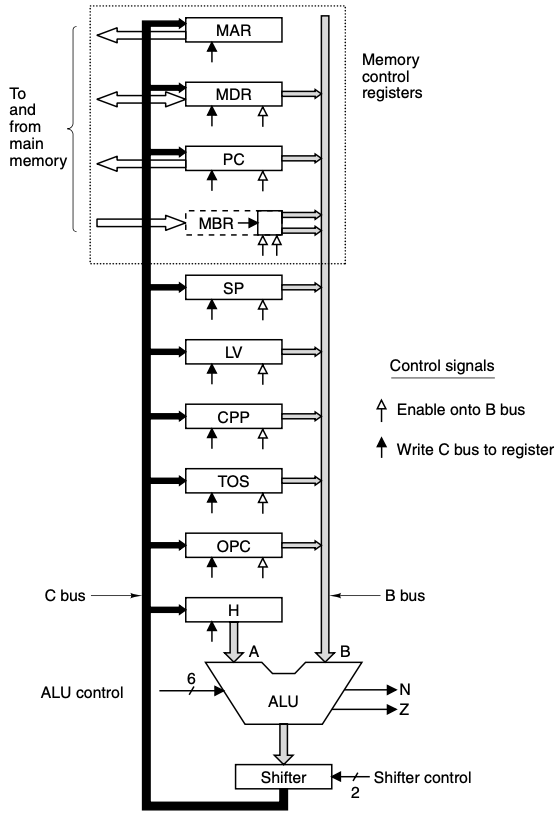
\includegraphics[width=0.9\textwidth]{datapath.png}
  \caption{Parte operativa del processore Mic-1}\label{fig:datapath}
\end{figure}

I registri hanno dimensione di 32 bit e non sono accessibili al programmatore,
ma solo al microprogramma.

\begin{mynote}{}{}
  Quando diciamo che i registri non sono accessibili al programmatore intendiamo
  che essi non fanno parte del \textit{modello di programmazione}, i.e.~non
  vengono utilizzati esplicitamente come operandi delle istruzioni. Vengono
  invece utilizzati dal microprogramma per implementare le istruzioni stesse.
\end{mynote}

L'unità operativa dispone di due bus, indicati con \lstinline{B} e
\lstinline{C}, collegati rispettivamente al secondo ingresso e all'uscita
dell'ALU; il primo ingresso dell'ALU è invece collegato esclusivamente al
registro \lstinline{H} (\textit{holding}).

Con alcune eccezioni (i cui motivi diverranno chiari a breve), i registri
dispongono di una coppia di segnali di controllo che permettono:
\begin{itemize}
    \item di abilitare il collegamento del registro al bus \lstinline{B},
    rendendolo effettivamente l'operando \lstinline{B} dell'ALU;
    \item di abilitare la scrittura sul registro del risultato fornito dall'ALU
    sul bus \lstinline{C}.
\end{itemize}

Solo un registro può essere collegato al bus \lstinline{B} in un determinato
istante, mentre il risultato dell'ALU (i.e.~il dato sul bus \lstinline{C}) può
essere scritto su più registri se necessario.

\begin{mynote}{}{}
  Il collegamento dei registri al bus \lstinline{B} può essere implementato
  usando porte tri-state o un multiplexer; nel nostro caso, useremo un
  multiplexer in quanto gli FPGA di cui facciamo uso dispongono di buffer
  tri-state esclusivamente ai pad di IO.
\end{mynote}

\subsection{L'Unità Aritmetico Logica}

L'ALU del processore Mic-1 ha due ingressi, che denominiamo \lstinline{A} e
\lstinline{B}; l'ingresso \lstinline{A} è collegato esclusivamente al registro
\lstinline{H}, mentre l'ingresso \lstinline{B} è collegato al bus
omonimo, che può essere guidato dalle nove sorgenti indicate con una freccia
grigia in fig.~\ref{fig:datapath}; le sue funzioni sono controllate mediante sei
linee di controllo, che consideriamo asserite se poste a 1:
\begin{itemize}
  \item \lstinline{F0} e \lstinline{F1} determinano l'operazione da eseguire;
  \item \lstinline{ENA} e \lstinline{ENB} abilitano singolarmente gli ingressi;
  \item \lstinline{INVA} inverte l'ingresso \lstinline{A};
  \item \lstinline{INC} incrementa di 1 il risultato.
\end{itemize}

Non tutte le combinazioni di questi segnali sono rilevanti; alcune delle più
importanti per implementare il set di istruzioni IJVM sono riportate in
tab.~\ref{fig:alu_func}.

\begin{figure}
  \centering
  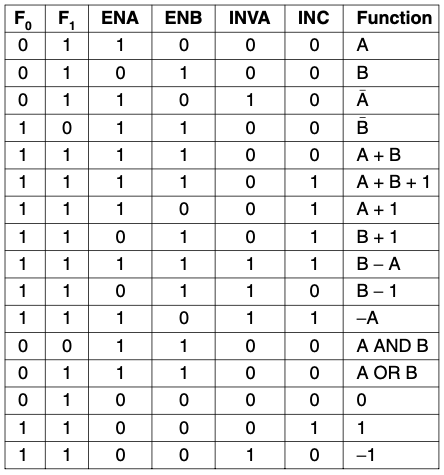
\includegraphics[width=0.6\textwidth]{alu_func.png}
  \caption{Segnali di controllo ALU e relative funzioni}\label{fig:alu_func}
\end{figure}

A questi segnali di controllo se ne aggiungono due ulteriori, utilizzati per
eseguire lo shift del risultato dell'ALU prima che esso venga posto sul bus
\lstinline{C}:
\begin{itemize}
  \item \lstinline{SLL8} (\textit{Shift Left Logical 8 bit}) esegue lo shift a
  sinistra di 8 bit, ponendo i bit meno significativi a \lstinline{0};
  \item \lstinline{SRA1} (\textit{Shift Right Arithmetic 1 bit}) esegue lo shift
  a destra di 1 bit, con estensione del segno (i.e. il bit più significativo non
  cambia).
\end{itemize}

Oltre a quella relativa al risultato, l'ALU dispone di due uscite \textit{flag}
ulteriori:
\begin{itemize}
  \item il flag \lstinline{N} è posto a 1 se il risultato è negativo;
  \item il flag \lstinline{Z} è posto a 1 se il risultato è 0.
\end{itemize}

\subsection{L'Interfaccia con la Memoria}

Il processore Mic-1 può comunicare con la memoria mediante due interfacce:
\begin{itemize}
  \item \lstinline{MAR} e \lstinline{MDR} controllano un'interfaccia
  word-addressable a 32 bit in lettura e scrittura;
  \item \lstinline{PC} e \lstinline{MBR} controllano un'interfaccia
  byte-addressable a 8 bit in sola lettura.
\end{itemize}

\begin{mynote}{}{}
  Come vedremo in seguito, la prima interfaccia è utilizzata per accedere ai
  dati su cui operano le istruzioni IJVM, rappresentati su 32 bit; la seconda,
  invece, per prelevare le istruzioni IJVM dalla memoria, che possono avere una
  lunghezza variabile in multipli di byte (e richiedono dunque più accessi
  successivi in memoria). Gli indirizzi sono comunque rappresentati su 32 bit
  per entrambe le interfacce.
\end{mynote}

Le due interfacce funzionano in modo simile in lettura: l'indirizzo da cui si
vuole leggere deve essere posto nel registro \lstinline{MAR} (\lstinline{PC});
al successivo fronte di salita del clock, il dato è disponibile nel registro
\lstinline{MDR} (\lstinline{MBR}). Indirizzano però in modo diverso la memoria:
scrivendo \lstinline{0x00000002} nel registro \lstinline{PC} e abilitando una
lettura, il byte all'indirizzo \lstinline{0x00000002} (i.e.~il byte di indirizzo
2) viene letto e posto negli 8 bit meno significativi del registro
\lstinline{MBR}; scrivendo lo stesso indirizzo nel registro \lstinline{MAR} e
abilitando una lettura, i 4 byte \lstinline{0x8}-\lstinline{0x11} (i.e.~la word
di indirizzo 2) vengono letti e posti nel registro \lstinline{MDR}.

L'interfaccia \lstinline{MAR}/\lstinline{MDR} dispone inoltre di un segnale di
\textit{write enable} (\lstinline{WE}) che, se asserito al fronte di salita di
clock, indica alla memoria di scrivere il dato contenuto in \lstinline{MDR}
all'indirizzo contenuto in \lstinline{MAR}.

\begin{figure}
  \centering
  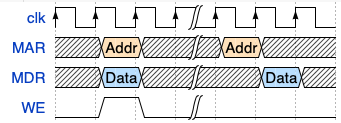
\includegraphics[width=0.5\textwidth]{mem_prot.png}
  \caption{Protocollo di scrittura e lettura sull'interfaccia
    \lstinline{MAR}/\lstinline{MDR}}\label{fig:mem_prot}
\end{figure}

Il protocollo per l'interfaccia a 32 bit è mostrato in fig.~\ref{fig:mem_prot}.

\subsection{Implementazione VHDL dell'Unità Operativa}

L'implementazione dell'unità operativa richiede di codificare in VHDL tre
parti principali:
\begin{itemize}
  \item i registri;
  \item i bus;
  \item l'ALU
\end{itemize}

\begin{mynote}{}{}
  Per il momento lasceremo in sospeso la struttura dell'entity relativa
  all'unità operativa, in quanto per capire quali segnali vengono esposti e
  perché è utile aver prima compreso anche il funzionamento dell'unità di
  controllo.
\end{mynote}

\subsubsection{Implementazione dei Registri}

I registri dell'unità operativa sono implementati mediante un singolo
\lstinline{process}, che ne gestisce la logica di reset e di scrittura mediante
il bus \lstinline{C}:

\begin{myvhdl}{datapath.vhd}
-- Registers
signal sp_reg   : reg_data_type;
signal lv_reg   : reg_data_type;
signal cpp_reg  : reg_data_type;

[...]

-- Processor registers
reg_proc : process(clk) is
begin
  if rising_edge(clk) then
    if reset = '1' then
      sp_reg  <= x"00000101";
      lv_reg  <= x"00000100";
      cpp_reg <= x"00000080";

      [...]

    else
      if c_to_reg_control(c_ctrl_mar) = '1' then
        mar_reg <= c_bus;
      end if;
      if c_to_reg_control(c_ctrl_pc) = '1' then
        pc_reg <= c_bus;
      end if;
      if c_to_reg_control(c_ctrl_sp) = '1' then
        sp_reg <= c_bus;
      end if;

      [...]

    end if;
  end if;
end process reg_proc;
\end{myvhdl}

Il tipo \lstinline{reg_data_type} è introdotto come abbreviazione per un
\lstinline{std_logic_vector} di 32 bit (\lstinline{31}:\lstinline{0}); è
definito, insieme ad altri tipi utili per l'implementazione del processore, nel
file \lstinline{common_defs.vhd}:

\begin{myvhdl}{common\_defs.vhd}
-- Data widths
--! Processor register data width
constant reg_data_width      : positive := 32;

[...]

-- Subtypes
--! Processor register data
subtype reg_data_type is std_logic_vector(reg_data_width - 1 downto 0);
\end{myvhdl}

Il segnale \lstinline{c_to_reg_control} è di tipo \lstinline{c_ctrl_type},
anch'esso definito nel file \lstinline{common_defs.vhd}, ed è indicizzato
mediante una serie di costanti relative agli indici dei singoli segnali di
attivazione:

\begin{myvhdl}{common\_defs.vhd}
--! C bus control width
constant c_ctrl_width        : positive := 9;

[...]

--! C bus control type
subtype c_ctrl_type is std_logic_vector(c_ctrl_width - 1 downto 0);

[...]

--! C control MAR bit
constant c_ctrl_mar        : natural := 0;
--! C control MDR bit
constant c_ctrl_mdr        : natural := 1;
--! C control PC bit
constant c_ctrl_pc         : natural := 2;
--! C control SP bit
constant c_ctrl_sp         : natural := 3;

[...]
\end{myvhdl}

\subsubsection{Implementazione dell'ALU}

In VHDL, l'\lstinline{entity} declaration per l'ALU che abbiamo descritto può
essere scritta come:

\begin{myvhdl}{alu.vhd}
entity alu is
  port (
    --! ALU control
    control       : in  alu_ctrl_type;
    --! ALU operand A
    operand_a     : in  reg_data_type;
    --! ALU operand B
    operand_b     : in  reg_data_type;
    --! ALU result
    sh_result     : out reg_data_type;
    --! Negative flag
    negative_flag : out std_logic;
    --! Zero flag
    zero_flag     : out std_logic
    );
end entity alu;
\end{myvhdl}

L'implementazione realizzata è puramente behavioral.

\subsubsection{Implementazione dei Bus}

In prima analisi, i bus sono implementati come dei \lstinline{signal}
VHDL:

\begin{myvhdl}{datapath.vhd}
-- Signals
signal a_bus : reg_data_type;
signal b_bus : reg_data_type;
signal c_bus : reg_data_type;
\end{myvhdl}

Punto critico nell'implementazione dei bus è però la disciplina di accesso
utilizzata. Per quanto riguarda \lstinline{A}, si tratta semplicemente
dell'insieme di fili che collega il registro \lstinline{H} al primo ingresso
dell'ALU; il bus \lstinline{C} invece è collegato all'uscita dello shifter della
componente ALU:

\begin{myvhdl}{datapath.vhd}
-- ALU instantiation
alu : entity work.alu
  port map (
    control       => alu_control,
    operand_a     => a_bus,
    operand_b     => b_bus,
    sh_result     => c_bus,
    negative_flag => alu_n_flag,
    zero_flag     => alu_z_flag);
\end{myvhdl}

Come abbiamo visto nella sezione relativa ai registri, il bus \lstinline{C} è
connesso a tutti i registri e un segnale di abilitazione per ciascuno di essi
funge da abilitazione in scrittura. Infine, il bus \lstinline{B} è implementato
mediante un multiplexer, implementato usando il costrutto VHDL
\lstinline{with/select} (\textit{selected assignment}):

\begin{myvhdl}{datapath.vhd}
with reg_to_b_control select b_bus <=
  mdr_reg         when b_ctrl_mdr,
  pc_reg          when b_ctrl_pc,
  mbr_s           when b_ctrl_mbr,
  mbr_u           when b_ctrl_mbru,
  sp_reg          when b_ctrl_sp,
  lv_reg          when b_ctrl_lv,
  cpp_reg         when b_ctrl_cpp,
  tos_reg         when b_ctrl_tos,
  opc_reg         when b_ctrl_opc,
  (others => '0') when others;
\end{myvhdl}

\section{Le Microistruzioni}

Per controllare l'unità operativa del processore, presentata in fig.
\ref{fig:datapath}, sono necessari 29 segnali:
\begin{itemize}
    \item 9 segnali per controllare la scrittura dei dati dal bus \lstinline{C}
    ai registri;
    \item 9 segnali per controllare quale registro è collegato al bus
    \lstinline{B} e va in ingresso all'ALU;
    \item 8 segnali per controllare l'ALU;
    \item 2 segnali per abilitare lettura/scrittura sull'interfaccia
    \lstinline{MAR}/\lstinline{MDR};
    \item 1 segnale per abilitare il fetch sull'interfaccia
    \lstinline{PC}/\lstinline{MBR}.
\end{itemize}

Poiché al più un registro alla volta può essere collegato al registro
\lstinline{B}, non c'è bisogno di utilizzare effettivamente 9 segnali: dato che
al più uno di essi può essere asserito, le 10 configurazioni possibili possono
essere codificate su $\ceil{\log_{2}10} = 4$ bit.

I 24 segnali individuati permettono di controllare l'unità operativa per un
ciclo di clock; per completare una microistruzione, è necessario aggiungere due
campi aggiuntivi, che chiamiamo \lstinline{Addr} e \lstinline{JAM}, che
descriveremo approfonditamente quando parleremo dell'unità di controllo; per il
momento, è sufficiente sapere che sono necessari a determinare la
microistruzione da eseguire nel ciclo di clock successivo.

\begin{figure}
  \centering
  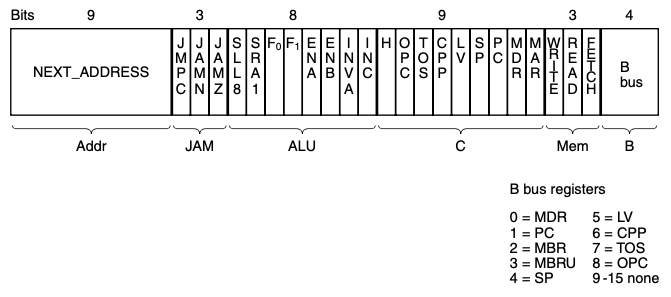
\includegraphics[width=\textwidth]{mu_instr.png}
  \caption{Il formato delle microistruzioni del Mic-1}\label{fig:mu_instr}
\end{figure}

In fig.~\ref{fig:mu_instr} è presentato il formato che adotteremo per le
microistruzioni, rappresentate su 36 bit; come anticipato, ogni microistruzione
comprende i seguenti campi:
\begin{itemize}
  \item \lstinline{Addr} - Indirizzo di una potenziale prossima microistruzione;
  \item \lstinline{JAM} - Determina come è selezionata la prossima
  microistruzione;
  \item \lstinline{ALU} - Controllo dell'ALU e dello shifter;
  \item \lstinline{C} - Controlla quali registri vengono scritti dal bus
  \lstinline{C};
  \item \lstinline{Mem} - Controlla le operazioni di memoria;
  \item \lstinline{B} - Seleziona il registro connesso al bus \lstinline{B}
  (codifica in fig.~\ref{fig:mu_instr}).
\end{itemize}

\subsection{Esempio pratico: l'istruzione \lstinline{IADD}}

Ora che abbiamo un'idea del funzionamento dell'unità operativa e della struttura
di una microistruzione, possiamo analizzare più nel dettaglio il modo in cui
viene eseguita un'istruzione IJVM. Consideriamo ad esempio l'istruzione
\lstinline{IADD}: quando l'abbiamo introdotta, abbiamo detto che ``esegue il pop
dei due elementi in cima allo stack e il push della loro somma''; questo
significa che il processore, in prima analisi, dovrebbe eseguire due accessi in
memoria in lettura, un'operazione di somma con l'ALU ed un accesso in memoria in
scrittura. In pratica, però, l'implementazione del microprogramma Mic-1 mantiene
due utili invarianti:
\begin{itemize}
  \item il registro \lstinline{SP} (\textit{Stack Pointer}), al termine dell'esecuzione
  di un'istruzione IJVM, contiene sempre l'indirizzo dell'elemento in testa allo
  stack;
  \item il registro \lstinline{TOS} (\textit{Top of Stack}), al termine dell'esecuzione
  di un'istruzione IJVM, contiene sempre il valore dell'elemento in testa allo
  stack.
\end{itemize}

È dunque sufficiente un singolo accesso in memoria, e l'istruzione può essere
eseguita in tre cicli di clock (i.e.~tre microistruzioni); supponendo che lo
stack si trovi nello stato in fig.~\ref{fig:stack_add}~(b), per quanto detto in
precedenza \lstinline{TOS} contiene il valore \lstinline{a3}; da questo stato:
\begin{enumerate}
  \item il contenuto di \lstinline{SP} viene decrementato di 1 e scritto sia in
  \lstinline{SP} che in \lstinline{MAR}, e si avvia l'operazione di lettura; si
  noti che \lstinline{SP} punta ora alla posizione da cui deve essere letto il
  valore di \lstinline{a2} e in cui in seguito sarà scritta la somma
  \lstinline{a2 + a3};
  \item il contenuto di \lstinline{TOS} è posto nel registro \lstinline{H};
  \item i dati contenuti in \lstinline{TOS} e \lstinline{MDR} (dato proveniente
  dalla memoria) sono sommati e posti sia in \lstinline{TOS} che in
  \lstinline{MDR}, si avvia una operazione di scrittura.
\end{enumerate}
È possibile verificare manualmente che queste operazioni rispettano le
invarianti enunciate in precedenza, e che il valore in cima allo stack è ora
proprio la somma dei due operandi che vi erano stati posti in precedenza.

Trascurando per ora i campi \lstinline{Addr} e \lstinline{JAM}, siamo in grado
di codificare gli altri campi delle microistruzioni:
\begin{enumerate}
  \item
  \begin{itemize}
    \item \lstinline{ALU}: \lstinline{110110} (decremento dell'operando \lstinline{B});
    \item \lstinline{C}: \lstinline{000001001} (bus \lstinline{C} scrive su
    \lstinline{SP} e \lstinline{MAR});
    \item \lstinline{Mem}: \lstinline{010} (lettura dati);
    \item \lstinline{B}: \lstinline{0100} (\lstinline{SP} controlla il bus \lstinline{B}).
  \end{itemize}
  \item
  \begin{itemize}
    \item \lstinline{ALU}: \lstinline{010100} (l'operando \lstinline{B} passa invariato);
    \item \lstinline{C}: \lstinline{100000000} (bus \lstinline{C} scrive su
    \lstinline{H});
    \item \lstinline{Mem}: \lstinline{000} (nessuna operazione di memoria);
    \item \lstinline{B}: \lstinline{0111} (\lstinline{TOS} controlla il bus \lstinline{B}).
  \end{itemize}
  \item
  \begin{itemize}
    \item \lstinline{ALU}: \lstinline{111100} (somma degli operandi
    \lstinline{A} e \lstinline{B});
    \item \lstinline{C}: \lstinline{001000010} (bus \lstinline{C} scrive su
    \lstinline{MDR} e \lstinline{TOS});
    \item \lstinline{Mem}: \lstinline{100} (scrittura dati);
    \item \lstinline{B}: \lstinline{0000} (\lstinline{MDR} controlla il bus \lstinline{B}).
  \end{itemize}
\end{enumerate}

\subsection{Il linguaggio MAL: parte 1}

Scrivere a mano le microistruzioni è perfettamente possibile, ma è molto
semplice commettere errori; inoltre, il microprogramma così ottenuto sarebbe
tedioso da comprendere e modificare.

\begin{figure}
  \centering
  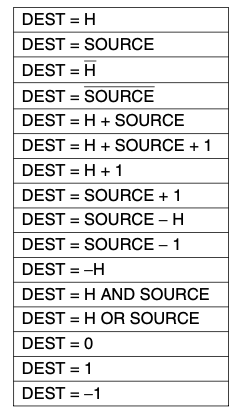
\includegraphics[width=0.3\textwidth]{mal_ops.png}
  \caption{Le operazioni permesse nel linguaggio MAL}\label{fig:mal_ops}
\end{figure}

Il linguaggio usato in~\cite{tanenbaum} per semplificare la scrittura del
microprogramma è denominato MAL (\textit{MicroAssembly Language}); un tool detto
\textit{microassemblatore} esegue dunque la traduzione nel formato di
fig.~\ref{fig:mu_instr}, completamente equivalente.

Introduciamo anzitutto la notazione necessaria a specificare il controllo dei
bus \lstinline{B} e \lstinline{C} e dell'ALU; le operazioni permesse sono
riportate in fig.~\ref{fig:mal_ops}, dove \lstinline{SOURCE} è uno dei registri
connessi al bus \lstinline{B} e \lstinline{DEST} una combinazione di registri
connessi al bus \lstinline{C}, eventualmente separati dal simbolo \lstinline{=};
ad esempio, per incrementare il contenuto del registro \lstinline{SP} e
scriverlo sia in \lstinline{SP} che in \lstinline{MAR}, si scrive:

\begin{lstlisting}
  SP = MAR = SP + 1
\end{lstlisting}

A ciascuna di queste operazioni può essere applicato uno shift a sinistra di 1 byte
aggiungendo \lstinline{<< 8}, ad esempio:

\begin{lstlisting}
  H = MBR << 8
\end{lstlisting}

Una seconda parte della microistruzione, separata dalla precedente da un punto e
virgola (\lstinline{;}), riguarda le istruzioni di memoria; lettura e scrittura
sull'interfaccia dati sono indicate rispettivamente da \lstinline{rd} o
\lstinline{wr}, mentre la lettura sull'interfaccia istruzioni è indicata da
\lstinline{fetch}; in una singola microistruzione è possibile avere
un'operazione per ciascuna delle due interfacce, eventualmente separate da
\lstinline{;}.

A questo punto siamo in grado effettivamente di tradurre in linguaggio MAL le
microistruzioni dell'istruzione \lstinline{IADD}:

\begin{lstlisting}
  MAR = SP = SP - 1; rd
  H = TOS
  MDR = TOS = MDR + H; wr
\end{lstlisting}

Questo frammento di microprogramma è tuttavia incompleto; per capire la funzione
dei campi \lstinline{Addr} e \lstinline{JAM} è necessario introdurre l'unità di
controllo del Mic-1.

\section{L'Unità di Controllo}

\begin{figure}
  \centering
  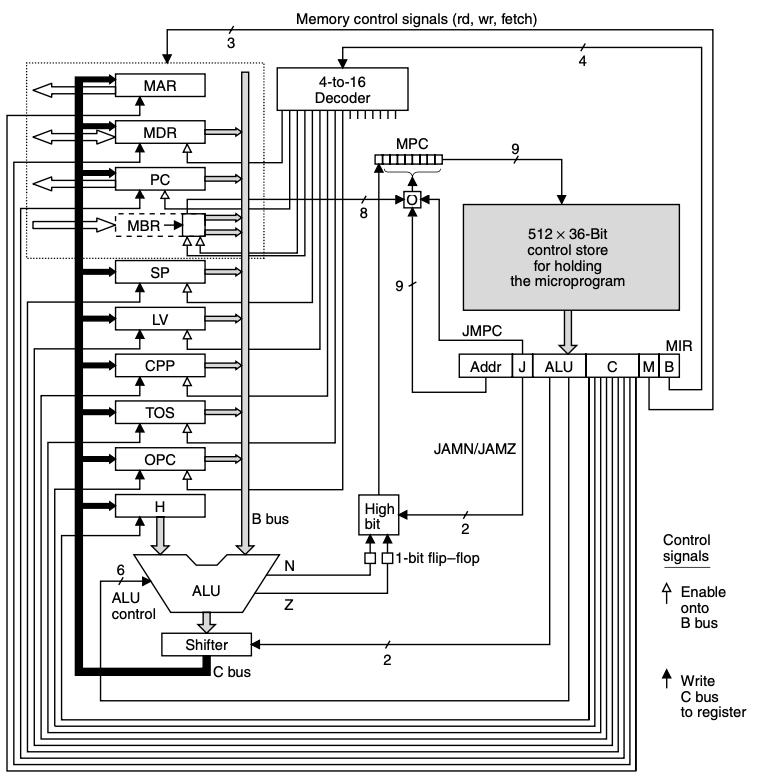
\includegraphics[width=\textwidth]{mic1.png}
  \caption{Diagramma completo del processore Mic-1}\label{fig:mic1}
\end{figure}

In fig.~\ref{fig:mic1} è riportato il diagramma completo del processore Mic-1,
in cui oltre all'unità operativa sono riportate le componenti dell'unità di
controllo.

L'unità di controllo del Mic-1 si comporta come un \textit{sequencer},
producendo in ciascun ciclo:
\begin{enumerate}
  \item lo stato dei segnali di controllo;
  \item l'indirizzo della prossima microistruzione da eseguire.
\end{enumerate}

Il microprogramma è effettivamente memorizzato in una memoria a sola lettura,
interna al processore, detta \textit{control store}; in pratica, il control
store contiene le microistruzioni del microprogramma allo stesso modo in cui la
memoria principale contiene le istruzioni (di livello ISA) del programma da
eseguire.

Anche l'accesso al control store richiede un'interfaccia, controllata dai due
registri \lstinline{MPC} (\textit{MicroProgram Counter}) e \lstinline{MIR}
(\textit{MicroInstruction Register}); non è necessario un segnale di lettura, in
quanto il control store è letto continuamente ad ogni ciclo.

Un'importante differenza è legata al fatto che, mentre le istruzioni del
programma sono eseguite generalmente in ordine sequenziale (a meno ovviamente di
istruzioni di salto), ciascuna microistruzione specifica esplicitamente
l'indirizzo della successiva, riportandolo nel campo \lstinline{Addr}.

Le microistruzioni forniscono tuttavia un supporto al controllo dei salti
mediante il campo \lstinline{JAM}; i due bit \lstinline{JAMN} e \lstinline{JAMZ}
sono combinati con i valori dei flag \lstinline{N} e \lstinline{Z} dell'ALU, e
permettono di modificare il bit più significativo dell'\lstinline{MPC}:

\begin{lstlisting}
  MPC[8] = (JAMZ AND Z) OR (JAMN AND N) OR Add[8]
\end{lstlisting}

Inoltre, se il bit \lstinline{JMPC} è asserito, gli 8 bit meno significativi di
\lstinline{MPC} sono messi in \lstinline{OR} bit-a-bit con gli 8 bit contenuti
nel registro \lstinline{MBR}.

\subsection{Il linguaggio MAL: parte 2}

Possiamo a questo punto introdurre le parti mancanti del linguaggio MAL;
osserviamo il microcodice completo per l'istruzione \lstinline{IADD}:

\begin{lstlisting}
  iadd = 0x65:
      MAR = SP = SP - 1; rd
      H = TOS
      MDR = TOS = MDR + H; wr; goto main
\end{lstlisting}

Abbiamo aggiunto una label, \lstinline{iadd}, che permette di identificare la
locazione del control store, seguita dall'indirizzo nel control store a partire
dal quale verra posizionato il microcodice seguente (dunque 0x65-0x67); in
assenza di indicazioni esplicite, il campo \lstinline{Addr} contiene
semplicemente l'indirizzo della microistruzione successiva (dunque in questo
caso, le prime due istruzioni, situate agli indirizzi 0x65 e 0x66 nel control
store, avranno campo \lstinline{Addr} posto rispettivamente a 0x66 e 0x67).

Consideriamo invece l'ultima microistruzione; abbiamo aggiunto un'ulteriore
parte alla microistruzione, che influenza il suo campo \lstinline{Addr}:

\begin{lstlisting}
  goto main
\end{lstlisting}

indica al programma microassemblatore, che traduce il linguaggio MAL nel formato
delle microistruzioni, che il campo \lstinline{Addr} per questa microistruzione
deve essere posto uguale all'indirizzo della microistruzione che ha come label
\lstinline{main}.

Osserviamo anche il microcodice relativo alla label \lstinline{main}:

\begin{lstlisting}
  main:
      PC = PC + 1; fetch; goto (MBR)
\end{lstlisting}

Questa microistruzione è particolarmente importante, in quanto ogni istruzione
IJVM si conclude tornando ad essa; la sua funziona è incrementare il program
counter, fare il fetch del successivo byte di istruzione e usare il contenuto
del registro \lstinline{MBR} come prossimo valore del microprogram counter; il
campo

\begin{lstlisting}
  goto (MBR)
\end{lstlisting}

è codificato usando il bit \lstinline{JMPC} nel campo \lstinline{JAM}.

È chiaro da quanto detto che l'indirizzo che assegniamo ad una istruzione IJVM
nel control store deve essere uguale alla sua codifica in linguaggio macchina
prodotta dall'assemblatore IJVM: l'istruzione \lstinline{IADD} è codificata come
\lstinline{0x65}, e memorizzata proprio all'indirizzo \lstinline{0x65} nel
control store; quando la microistruzione \lstinline{main} esegue il fetch del
byte \lstinline{0x65}, l'\lstinline{MPC} è settato a \lstinline{0x65} e il
microcodice relativo all'istruzione \lstinline{IADD} viene eseguito.

Per concludere, il controllo di flusso basato sui flag dell'ALU è scritto in
linguaggio MAL come:

\begin{lstlisting}
  if (flag) goto T; else goto F
\end{lstlisting}

dove \lstinline{flag} può essere \lstinline{N} o \lstinline{Z}, mentre
\lstinline{T} e \lstinline{F} sono due label.

\subsection{Implementazione dell'Unità di Controllo}

Il control store presenta un'interfaccia molto semplice:

\begin{myvhdl}{control\_store.vhd}
entity control_store is
  port (
    --! Address of the desired word
    address : in  ctrl_str_addr_type;
    --! Content of the addressed word
    word    : out ctrl_str_word_type
    );
end entity control_store;
\end{myvhdl}

Le microistruzioni sono inserite direttamente all'interno del codice:

\begin{myvhdl}{control\_store.vhd}
constant words : ctrl_str_type := (
--BEGIN_WORDS_ENTRY
0 => "000000110000000000000000000000001001",
1 => "010111100000000000000000000000001001",
2 => "000000000000000000000000000000000000",

[...]

--END_WORDS_ENTRY
);
\end{myvhdl}

Tutti i tipi sono definiti, come negli altri casi, nel file
\lstinline{common\_defs.vhd}:

\begin{myvhdl}{common\_defs.vhd}
--! Control store address
subtype ctrl_str_addr_type is std_logic_vector(ctrl_str_addr_width - 1 downto 0);
--! Control store word
subtype ctrl_str_word_type is std_logic_vector(ctrl_str_word_width - 1 downto 0);

[...]

--! Control store word
subtype ctrl_str_word_type is std_logic_vector(ctrl_str_word_width - 1 downto 0);

[...]

--! Control store content
type ctrl_str_type is array (ctrl_str_words - 1 downto 0) of ctrl_str_word_type;
\end{myvhdl}

L'implementazione della control unit è molto semplice: un \lstinline{process}
aggiorna il registro \lstinline{MIR} con la microistruzione corrente, i cui bit
del campo \lstinline{Addr}, opportunamente mascherati, costituiscono il registro
``virtuale'' \lstinline{MPC}:

\begin{myvhdl}{control\_unit.vhd}
-- Registers
reg_proc : process(clk) is
begin
  if rising_edge(clk) then
    if reset = '1' then
      mir_reg <= "000000001000000000000000000000001001";
      n_ff    <= '0';
      z_ff    <= '0';
    else
      mir_reg <= control_store_word;
      n_ff    <= alu_n_flag;
      z_ff    <= alu_z_flag;
    end if;
  end if;
end process reg_proc;

-- MPC virtual register
ctrl_nxt_addr_no_msb <= mir_reg(ctrl_nxt_addr_no_msb_type'range);
jmpc_addr <= ctrl_nxt_addr_no_msb or mbr_reg_in when mir_reg(ctrl_jmpc) = '1' else ctrl_nxt_addr_no_msb;
high_bit <= (alu_n_flag and mir_reg(ctrl_jamn)) or (alu_z_flag and mir_reg(ctrl_jamz));
mpc_virtual_reg <= (mir_reg(ctrl_nxt_addr_msb) or high_bit) & jmpc_addr;
\end{myvhdl}

Il decoder per la selezione del registro che controlla il bus \lstinline{B} è
implementato come un \lstinline{process} puramente combinatorio:
\begin{myvhdl}{control\_unit.vhd}
-- B_BUS control decoder
reg_to_b_decoder : process(mir_reg(ctrl_b'range)) is
begin
  reg_to_b_decoder_out <= (others => '0');

  if unsigned(mir_reg(ctrl_b'range)) < b_ctrl_width then
    reg_to_b_decoder_out(to_integer(
      unsigned(mir_reg(ctrl_b'range)))) <= '1';
  end if;
end process reg_to_b_decoder;
\end{myvhdl}

\subsection{Collegarmento tra UO e UC}

Siamo finalmente in grado di definire le \lstinline{entity} relative all'unità
operativa e all'unità di controllo.

Entrambe le unità devono ricevere:
\begin{itemize}
  \item un segnale di clock;
  \item un segnale di reset.
\end{itemize}
Questi segnali sono comuni.

L'unità di controllo fornisce all'unità operativa i segnali relativi:
\begin{itemize}
  \item al controllo dell'ALU;
  \item al controllo del bus \lstinline{C};
  \item al controllo del bus \lstinline{B};
  \item al controllo della memoria.
\end{itemize}

Riceve invece da essa:
\begin{itemize}
  \item i flag dell'ALU;
  \item il contenuto del registro \lstinline{MBR}.
\end{itemize}

\begin{myvhdl}{control\_unit.vhd}
 entity control_unit is
  port (
    --! Clock
    clk              : in  std_logic;
    --! Synchronous active-high reset
    reset            : in  std_logic;
    --! Content of the MBR register
    mbr_reg_in       : in  mbr_data_type;
    --! ALU negative flag
    alu_n_flag       : in  std_logic;
    --! ALU zero flag
    alu_z_flag       : in  std_logic;
    --! Control signals for the ALU
    alu_control      : out alu_ctrl_type;
    --! Control signals for the C bus
    c_to_reg_control : out c_ctrl_type;
    --! Control signals for memory operations
    mem_control      : out mem_ctrl_type;
    --! Control signals for the B bus
    reg_to_b_control : out b_ctrl_type
    );
end entity control_unit;
\end{myvhdl}

In aggiunta a questi segnali, ci aspettiamo di trovare nell'\lstinline{entity}
dell'unità operativa anche i porti relativi all'interfaccia con la memoria:
\begin{itemize}
  \item indirizzo dati;
  \item ingresso dati;
  \item uscita dati;
  \item write enable dati;
  \item indirizzo istruzioni;
  \item ingresso istruzioni.
\end{itemize}

\begin{myvhdl}{datapath.vhd}
entity datapath is
  port (
    --! Clock
    clk              : in  std_logic;
    --! Synchronous active-high reset
    reset            : in  std_logic;
    --! Control signals for the ALU
    alu_control      : in  alu_ctrl_type;
    --! Control signals for the C bus
    c_to_reg_control : in  c_ctrl_type;
    --! Control signals for memory operations
    mem_control      : in  mem_ctrl_type;
    --! Control signals for the B bus
    reg_to_b_control : in  b_ctrl_type;
    --! Content of the MBR register
    mbr_reg_out      : out mbr_data_type;
    --! ALU negative flag
    alu_n_flag       : out std_logic;
    --! ALU zero flag
    alu_z_flag       : out std_logic;
    --! Memory data write enable
    mem_data_we      : out std_logic;
    --! Port for memory data read
    mem_data_in      : in  reg_data_type;
    --! Port for memory data write
    mem_data_out     : out reg_data_type;
    --! Memory address for memory data operations
    mem_data_addr    : out reg_data_type;
    --! Port for memory instruction read
    mem_instr_in     : in  mbr_data_type;
    --! Memory address for memory instruction fetch
    mem_instr_addr   : out reg_data_type
    );
end entity datapath;
\end{myvhdl}

Infine, introduciamo il componente \lstinline{processor} all'interno del quale
sono istanziati sia il \lstinline{datapath} che la \lstinline{control_unit}.
Tutte le coppie di porti corrispondenti sono connesse internamente, mentre sono
esposti quelli relativi:
\begin{itemize}
  \item al clock;
  \item al reset;
  \item all'interfaccia con la memoria.
\end{itemize}

\begin{myvhdl}{processor.vhd}
entity processor is
  port (
    --! Clock
    clk            : in  std_logic;
    --! Synchronous active-high reset
    reset          : in  std_logic;
    --! Memory data write enable
    mem_data_we    : out std_logic;
    --! Port for memory data read
    mem_data_in    : in  reg_data_type;
    --! Port for memory data write
    mem_data_out   : out reg_data_type;
    --! Memory address for memory data operations
    mem_data_addr  : out reg_data_type;
    --! Port for memory instruction read
    mem_instr_in   : in  mbr_data_type;
    --! Memory address for memory instruction fetch
    mem_instr_addr : out reg_data_type
    );
end entity processor;
\end{myvhdl}

\chapter{La Toolchain Mic-1}

\section{Installazione}

Per installare il microassemblatore \lstinline{mal} e l'assemblatore
\lstinline{ajvm} è anzitutto necessario installare il version control system Git
ed il build system Gradle; inoltre, per alcuni task useremo il build system
Cmake. La procedura può variare leggermente a seconda del sistema operativo
usato, ma in una tipica distribuzione Linux Debian-based (come Ubuntu) è
sufficiente eseguire:

\begin{commandshell}
sudo apt install git gradle cmake
\end{commandshell}

Conviene dunque creare una nuova cartella per i repository da scaricare, e
posizionarvici; al suo interno, creeremo anche una directory per i tool compilati:

\begin{commandshell}
mkdir esercitazione_mic
cd esercitazione_mic
mkdir tools
\end{commandshell}

È possibile a questo punto compilare i tool (ignorando eventuali warning in fase
di test):

\begin{commandshell}
git clone https://github.com/albmoriconi/mal.git
cd mal
./gradlew build
cd ..
git clone https://github.com/albmoriconi/ajvm.git
cd ajvm
./gradlew build
cd ..
tar -xvf mal/build/distributions/mal.tar -C tools/
tar -xvf ajvm/build/distributions/ajvm.tar -C tools/
\end{commandshell}

Per poter usare i tool nella shell attiva, le loro directory vanno aggiunte al
path di ricerca dei binari; il comando seguente può essere aggiunto al proprio
profilo della shell o eseguito direttamente da riga di comando (in questo caso,
deve essere eseguito nuovamente ogni volta che si apre una nuova shell, o i tool
non saranno trovati):

\begin{lstlisting}
  PATH="$HOME/esercitazione_mic/tools/ajvm/bin:$HOME/esercitazione_mic/tools/mal/bin:$PATH"
\end{lstlisting}

Infine, è possibile eseguire il clone del repository contenente il codice VHDL
del processore, e predisporne la directory per la build:

\begin{commandshell}
  git clone https://github.com/albmoriconi/amic-0.git
  cd amic-0
  mkdir build
  cd build
  cmake ..
\end{commandshell}

\section{Struttura del Progetto}

Da qui in avanti, ogni volta che faremo riferimento a un percorso sarà rispetto
alla directory in cui è stato scaricato il repository \lstinline{amic-0}.

La directory principale del repository è organizzata come segue:
\begin{itemize}
  \item \lstinline{src} - codice sorgente
  \begin{itemize}
    \item \lstinline{main} - implementazione (subdirectory ordinate per
    linguaggio)
    \item \lstinline{test} - testbench (subdirectory ordinate per linguaggio)
  \end{itemize}
  \item \lstinline{util} - utility necessarie per il flow di sviluppo
  (subdirectory ordinate per linguaggio)
  \item \lstinline{build} - contiene i file prodotti dal build system (questa
  directory deve essere creata manualmente)
\end{itemize}

Per il momento non ci interessano le altre directory e file presenti; è
importante tuttavia notare che ogni directory che contiene codice (eventualmente
nelle subdirectory) contiene anche un file \lstinline{CMakeLists.txt} che serve
al build system per tenere traccia dei sorgenti e aggiungerli ai target
opportuni.

\section{Flow di Sviluppo}

Per utilizzare il flow di sviluppo da linea di comando è necessario installare
due tool aggiuntivi: il simulatore \lstinline{ghdl} e il visualizzatore di forme
d'onda \lstinline{gtkwave}:

\begin{commandshell}
  sudo apt install ghdl gtkwave
\end{commandshell}

Dalla directory build è ora possibile lanciare il tool \lstinline{make} con una
serie di target utili per lanciare microassemblatore, assemblatore e alcuni
test.

In particolare, è possibile editare il microprogramma in linguaggio MAL e il
programma in linguaggio IJVM situati rispettivamente nelle directory
\lstinline{src/main/mal} e \lstinline{src/main/ajvm} e dunque rigenerare control
store e RAM lanciando, dalla directory \lstinline{build}, i target:

\begin{commandshell}
  make create_control_store
  make create_ram
\end{commandshell}

Il target \lstinline{check} lancia invece i testbench contenuti nella directory
\lstinline{src/test/vhdl}:
\begin{commandshell}
  make check
\end{commandshell}

Un esempio dei risultati della suite di test è riportato in
fig.~\ref{fig:test}. L'esecuzione dei test produce anche le waveform relative
alle esecuzioni dei testbench, come quella riportata in fig.~\ref{fig:waveform},
che possono essere trovate nella directory \lstinline{build/src/test/vhdl} e
visualizzate utilizzando il tool \lstinline{gtkwave}.

Per aggiungere altri testbench alla suite è sufficiente salvarli nella
directory \lstinline{test/vhdl} e modificare il file
\lstinline{test/vhdl/CmakeLists.txt} aggiungendo alla macro
\lstinline{add_vhdl_test_sources} un'entry relativa al nuovo testbench.

\begin{figure}
  \centering
  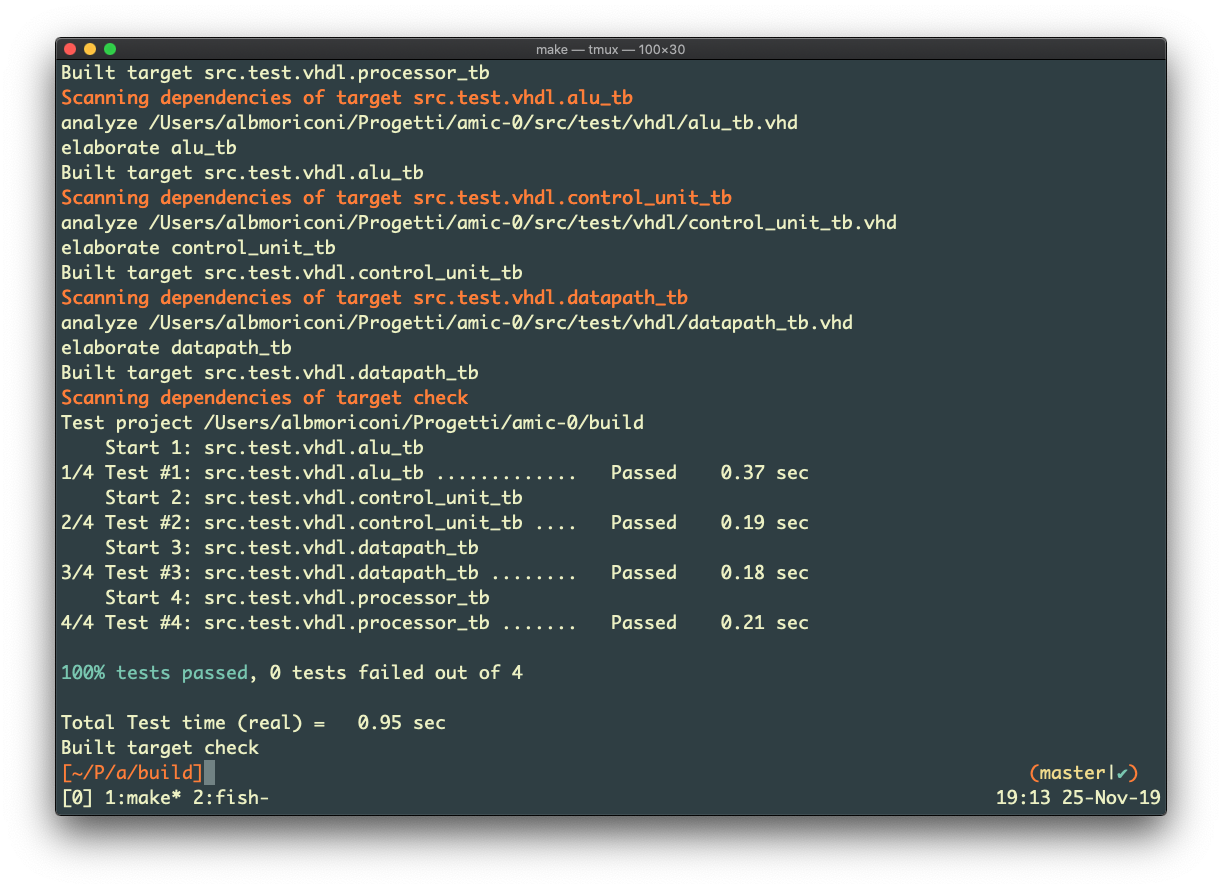
\includegraphics[width=0.8\textwidth]{test.png}
  \caption{Risultati dei testbench}\label{fig:test}
\end{figure}

\begin{figure}
  \centering
  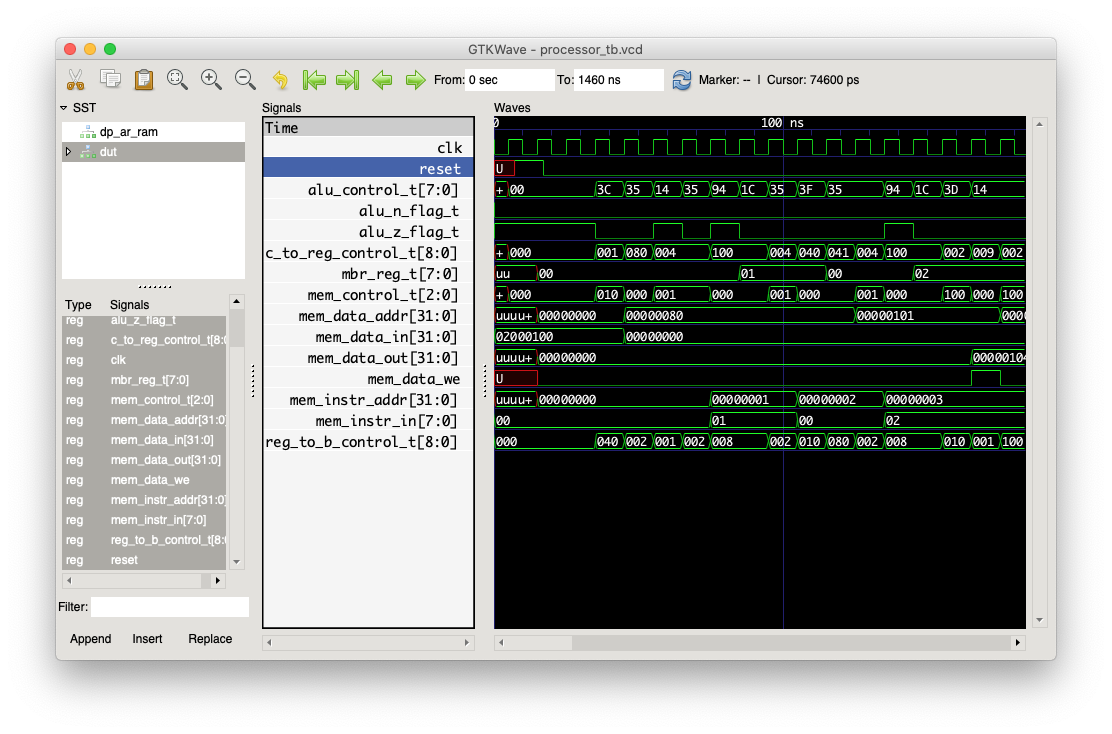
\includegraphics[width=0.8\textwidth]{waveform.png}
  \caption{Waveform del testbench \lstinline{processor_tb.vhd}}\label{fig:waveform}
\end{figure}

\begin{thebibliography}{2}
  \bibitem{tanenbaum}
  Andrew S. Tanenbaum and Todd Austin.
  \textit{Structured Computer Organization}.
  Pearson, 2013.

  \bibitem{calc}
  Gianni Conte, Antonino Mazzeo, Nicola Mazzocca and Paolo Prinetto.
  \textit{Architettura dei Calcolatori}.
  CittàStudi, 2015.
\end{thebibliography}
\end{document}
